\documentclass[aspectratio=169, 12pt]{beamer}
\usepackage{bbm}
\usepackage[utf8]{inputenc}
\usepackage[T2A]{fontenc}
\usepackage[english]{babel}
\usepackage{amscd,amssymb}
\usepackage{amsfonts,amsmath,array}
\usepackage{sidecap}
\usepackage[T2A]{fontenc}
\usepackage[utf8]{inputenc}
\usepackage{graphicx}				% Вставка картинок правильная
\graphicspath{{pictures/}, {images/}, {}}
\DeclareGraphicsExtensions{.pdf,.png,.jpg}
\usepackage{pdfpages}
\usepackage{multicol}

% Для алгоритмов
\usepackage{algorithm}
\usepackage{algpseudocode}
% Цвета 
\usepackage{color}
\usepackage{colortbl}

% Создаем новую команду для assumptions
%----------------------------------------------------------------------------------------------------------
\newtheorem*{assumption*}{\assumptionnumber}
\providecommand{\assumptionnumber}{}
\makeatletter
\newenvironment{assumption}[2]
 {%
  \renewcommand{\assumptionnumber}{\textbf{Assumption} #1 ({#2})}%
  \begin{assumption*}%
  \protected@edef\@currentlabel{#1-#2}%
 }
 {%
  \end{assumption*}
 }

%beamer  theme's used to be here :)
%\usetheme{mipt_beamer}
\usetheme{boxes}

%----------------------------------------------------------------------------------------------------------
\title[\hbox to 56mm{Feature}]{Methods with preconditioning with weight decay regularization}
\author[M.\,K.~Kreinin]{Matvei Kreinin}
\institute{Moscow Institute of Physics and Technology}
\date{\footnotesize
\par\smallskip\emph{Course:} My first scientific paper\par (Strijov's practice)/Group 003 %821, 813
\par\smallskip\emph{Expert:} A. Beznosikov
\par\bigskip\small 2023}

\begin{document}
\maketitle
\begin{frame}{Goal of researches}
    \textbf{Goal objectives:} create new method of optimization and investigate theory and practical convergence of algorithms.

    \textbf{Problem:} 
    \begin{itemize}
        \item Prove the convergence of the methods with preconditioning with weight decays.
        \item Research the  convergence on practical tasks.
        \item Create and investigate new optimization algorithm 
        \item Compare it with the others
    \end{itemize}
\end{frame}

\begin{frame}{Notation}
\begin{itemize}
    \item Minimization problem:
    $$ \min_{x \in \mathbb{R}^d} f(x) $$
    
    
    \item $r(x)$ -- regularization function, $r(x) = \frac{\lambda}{2} ||x||_2^2$
    \item methods with preconditioning
$$
    w_t = w_{t-1} - \eta \cdot D_t^{-1} g_t,
$$
    
    \item New regularization function $\tilde{r}(x) :$ $\nabla \tilde{r}(x) = D_t \nabla r(x)$

    \item New objective function $\tilde{F}(x) = f(x) + \tilde{r}(x) $
    
\end{itemize}
\end{frame}

\begin{frame}{Assumptions}
    \begin{assumption}{1}{Convex}
	The function f is convex, i.e. $\forall x, y \in \mathbb{R}^d$
	\begin{equation*}
		f(y) \geq f(x) + \langle \nabla f(x), y-x \rangle
	\end{equation*}
\end{assumption}
\begin{assumption}{2}{PL--condition}
	If there exists $\mu > 0$, such that $||\nabla f(w) || \geq 2 \mu (f(w) - f^*)$, $\forall w \in \mathbb{R}^d$
\end{assumption}

\end{frame}


\begin{frame}{Assumptions}
\begin{assumption}{3}{L-l-smoothness}
The gradients of F are L-Lipschitz continuous $\forall w \in \mathbb{R}^d$, i.e. there exists a constant $L > 0$ such that $\forall x, y \in \mathbb{R}^d$,
	\begin{equation*}
		f(x) \leq f(y) + \langle \nabla f(y), x-y \rangle + \frac{L}{2} ||x - y||^2
	\end{equation*}

    The gradient of r is l-Lipschitz continuous $\forall w \in \mathbb{R}^d$, i.e. there exists a constant $l > 0$ such that $\forall x, y \in \mathbb{R}^d$,
	\begin{equation*}
		r(x) \leq r(y) + \langle \nabla r(y), x-y \rangle + \frac{l}{2} ||x - y||^2
	\end{equation*}
\end{assumption}

\end{frame}

\begin{frame}{Differen ways of regularization}
\begin{algorithm}[H]
    \caption{Different ways of regularization}
    \label{alg:precond}
    
    \begin{algorithmic}
            \Require{$\eta, f$}
            
            \While {$w$ not converged}
            \State $t = t+1$
            \State $g_t \gets$ stochastic gradient
            \State $\textcolor{blue}{g_t \gets g_t + \nabla r(w_t)}$ \hfill \textcolor{blue}{standart regularization}
            \State $D_t \gets$ preconditioning matrix
            \State $w_t \gets w_{t-1} - \eta \cdot D_t^{-1} \left(g_t +\textcolor{orange}{\nabla r(w_t)} \right) \textcolor{red}{ - \eta \cdot \nabla r(w_t)}$ \hfill \textcolor{orange}{hessian weight decay}, \textcolor{red}{weight decay}
            \EndWhile
    \end{algorithmic}
\end{algorithm}
\end{frame}

\begin{frame}{Theorem №1}
\begin{theorem}[1]
Suppose the Assumption 1, 3 and let $\varepsilon > 0$ and let the step-size satisfy
\begin{equation*}
    \eta < \frac{2 \alpha}{L + l \cdot \alpha} 
\end{equation*}
Then, the number of iterations performed by algorithm, starting from an initial point $w_0 \in \mathbb{R}^d$ with $\Delta_0 = \tilde{F}(w_0) - \tilde{F}^*$, required to obtain and $\varepsilon$-approximate solution of the problem can be bounded by
\begin{equation*}
      T = \mathcal{O}\left( \frac{2\Delta_0 \Gamma \alpha } {(2\alpha - \tilde{L}\eta) \eta \varepsilon} \right)
\end{equation*}

\end{theorem}
\end{frame}
\begin{frame}{Proof Theorem №1 (1/4)}
    
Let's write first assumption for step t and $t+1$:

\begin{equation*}
    f(w_{t+1}) \leq f(w_t) + \langle \nabla f(w_t), w_{t+1} - w_t \rangle + \frac{L}{2}||w_{t+1} - w_t ||^2,
\end{equation*}
Okay, by definition for our algorithm we have:

\begin{equation*}
w_{t+1} - w_t = -\eta D_t^{-1} \nabla f(w_t) - \eta \nabla r(w_t),
\end{equation*}
and 

\begin{equation*}
\nabla f(w_t) = \frac{1}{\eta} D^t(w_t - w_{t+1}) - D^t \nabla r(w_t),
\end{equation*}

\end{frame}

\begin{frame}{Proof Theorem №1 (2/4)}
    Okay, now let's replace $\nabla f(w_t)$ and $I \leq \frac{D_t}{\alpha}$
\begin{equation*}
    f(w_{t+1}) \leq f(w_t) + \langle \frac{1}{\eta}D_t(w_t - w_{t+1}) - D_t\nabla r(w_t), w_{t+1} - w_t \rangle + \frac{L}{2 \alpha} ||w_{t+1} - w_t||_{D_t}^2,
\end{equation*}

\begin{equation*}
    f(w_{t+1}) \leq f(w_t) + \left(\frac{L}{2 \alpha} - \frac{1}{\eta} \right) ||w_{t+1} - w_t||_{D_t}^2 - \langle D_t \nabla r(w_t), w_{t+1} - w_t \rangle,
\end{equation*}

Lets define new variable $\tilde{r} : \nabla \tilde{r} = D_t \nabla r(w_t)$. Then rewrite step using the variable and 5-th assumption.
\begin{equation*}
    \tilde{r}(w_{t+1}) \leq \tilde{r}(w_t) + \langle \tilde{r}(w_t), w_{t+1} - w_t \rangle + \frac{l}{2} (w_{t+1} - w_t)^T D_t (w_{t+1} - w_t),
\end{equation*}
\end{frame}

\begin{frame}{Proof Theorem №1 (3/4)}
    \begin{equation*}
    f(w_{t+1}) \leq f(w_t) + \left( \frac{L}{2\alpha} - \frac{1}{\eta} \right) ||w_{t+1} - w_t||_{D_t}^2 + \tilde{r}(w_t) - \tilde{r}(w_{t+1}) + \frac{l}{2}||w_{t+1}-w_t||_{D_t}^2,
\end{equation*}

$\tilde{F}(w) = f(w) + \tilde{r}(w)$, $F(w) = f(w) + r(w)$, ($\tilde{L}=L + l \alpha$), we get:

\begin{equation*}
    \tilde{F}(w_{t+1}) \leq \tilde{F}(w_t) + \left( \frac{\tilde{L}}{2\alpha} - \frac{1}{\eta}  \right) ||w_{t+1} - w_t||_{D_t}^2,
\end{equation*}


\begin{equation*}
    \left(\frac{1}{\eta} - \frac{\tilde{L}}{2\alpha}   \right) ||w_{t+1} - w_t||_{D_t}^2 \leq \tilde{F}(w_t) - \tilde{F}(w_{t+1})
\end{equation*}
\end{frame}

\begin{frame}{Proof Theorem №1 (4/4)}
\begin{eqnarray*}
&& \frac{\eta^2  (T+1)}{\Gamma}\left(\frac{1}{\eta} - \frac{\tilde{L}}{2\alpha}   \right)\cdot\min_{k = 0, T} ||\nabla f(w_t) + \nabla \tilde{r}(w_t)||^2 \leq
\notag\\&\leq&
\frac{\eta^2}{\Gamma}\left(\frac{1}{\eta} - \frac{\tilde{L}}{2\alpha}   \right)\cdot\sum\limits_{t = 0}^T ||\nabla f(w_t) + \nabla \tilde{r}(w_t)||^2 \leq \tilde{F}(w_0) - \tilde{F}(w_*),    
\end{eqnarray*}

\begin{equation*}
    \min_{t = 0, T} ||\nabla f(w_t) + \nabla \tilde{r}(w_t)||^2 \leq \frac{(\tilde{F}(w_0) - \tilde{F}(w_*))\Gamma}{(\frac{1}{\eta} - \frac{\tilde{L}}{2\alpha}) \eta^2 (T+1)} = \varepsilon,
\end{equation*}

\begin{equation*}
    T + 1 \geq \frac{\Delta_0 \Gamma}{(\frac{1}{\eta} - \frac{\tilde{L}}{2\alpha}) \eta^2 \varepsilon}
\end{equation*}
    Then:
\begin{equation*}
      T = \mathcal{O}\left( \frac{2\Delta_0 \Gamma \alpha } {(2\alpha - \tilde{L}\eta) \eta \varepsilon} \right)
\end{equation*}
\end{frame}

\begin{frame}{Theorem №2}
    \begin{theorem}
    Suppose the Assumption 1, 2, 3 and let $\varepsilon > 0$ and let the step-size satisfy
    \begin{equation*}
        \eta \leq \frac{2 \alpha}{\tilde{L}}
    \end{equation*}
    Then, the number of iterations performed by algorithm, starting from an initial point $w_0 \in \mathbb{R}^d$ with $\Delta_0 = \tilde{F}(w_0) - \tilde{F}^*$, required to obtain and $\varepsilon$-approximate solution of the problem can be bounded by
    \begin{equation*}
        T =  \mathcal{O}\left( \frac{\ln \frac{\Delta_0}{\epsilon}}{2 \mu \eta^2(\frac{1}{\eta} - \frac{\tilde{L}}{2 \alpha})} \right)
    \end{equation*}
\end{theorem}
\end{frame}

\begin{frame}{Proof Theorem №2}
        Assume 
    \begin{equation*}
    \nabla \tilde{F} = \nabla f + \nabla \tilde{r}    
    \end{equation*}
    
    \begin{equation*}
    L + ||D_t||l = \tilde{L}        
    \end{equation*}
    
    \begin{equation*}
    w_{t+1} - w_t = -\eta D_t^{-1} \nabla r(w_t) - \eta \nabla r(w_t) = -\eta D_t^{-1} (\nabla f + \nabla \tilde{r})(w_t) = -\eta D_t^{-1} \nabla \tilde{F}(w_t)    
    \end{equation*}
    
    Then we write $\tilde{L}$-smoothness for $\tilde{F}$ 
    \begin{equation*}
        \tilde{F}(w_{t+1}) - \tilde{F}(w_t) \leq  \langle \nabla \tilde{F}(w_t), w_{t+1} - w_t \rangle + \frac{\tilde{L}}{2} ||w_{t+1} - w_t||^2
    \end{equation*}

    
\end{frame}

\begin{frame}{Proof Theorem №2}
    \begin{eqnarray*}
    &&
    \tilde{F}(w_{t+1}) - \tilde{F}(w_t) \leq - \langle \frac{1}{\eta} D_t(w_{t+1} - w_t), w_{t+1} - w_t \rangle + \frac{\tilde{L}}{2} ||w_{t+1} - w_t||^2 = 
    \notag\\&\ = &
    (\frac{\tilde{L}}{2 \alpha} - \frac{1}{\eta}) ||w_{t+1} - w_t||^2_{D_t} = (\frac{\tilde{L}}{2 \alpha} - \frac{1}{\eta}) ||-\eta D_t^{-1} \nabla \tilde{F}(w_t)||_{D_t}^2 \leq
    \notag\\&\ \leq &  (\frac{\tilde{L}}{2 \alpha} - \frac{1}{\eta}) \eta^2 ||\nabla \tilde{F}(w_t)||^2_{D_t^{-1}}
    \end{eqnarray*}
    
    Then we use PL-condition for the function $\tilde{F}$:
    \begin{equation*}
        ||\nabla \tilde{F}(w_t)||_{D_t^{-1}}^2 \geq 2 \mu (\tilde{F}(w_t) - \tilde{F}^*)
    \end{equation*}
\end{frame}

\begin{frame}{Proof Theorem №2}
    \begin{eqnarray*}
&& \tilde{F}(w_{t}) -  F^* \ge \tilde{F}(w_{t+1}) - \tilde{F}^* + (\frac{1}{\eta} - \frac{\tilde{L}}{2 \alpha}) \eta^2 2 \mu (\tilde{F}(w_t) - \tilde{F}^*)=
\notag\\&\ = & \left( 1 +  2 \mu \eta^2(\frac{1}{\eta} - \frac{\tilde{L}}{2 \alpha}) \right) (\tilde{F}(w_{t+1}) - \tilde{F}^*),    
\end{eqnarray*}
    
    \begin{equation*}
    \epsilon \ge \Delta_0 \left( 1 +  2 \mu \eta^2(\frac{1}{\eta} - \frac{\tilde{L}}{2 \alpha}) \right)^{-T} \ge (\tilde{F}(w_{T}) - \tilde{F}^*)        
    \end{equation*}

    \begin{equation*}
    T = \frac{\ln \frac{\Delta_0}{\epsilon}}{\ln(1 + 2 \mu \eta^2(\frac{1}{\eta} - \frac{\tilde{L}}{2 \alpha}))} \approx \frac{\ln \frac{\Delta_0}{\epsilon}}{2 \mu \eta^2(\frac{1}{\eta} - \frac{\tilde{L}}{2 \alpha})}        
    \end{equation*}
    Then:
    \begin{equation*}
    T =  \mathcal{O}\left( \frac{\ln \frac{\Delta_0}{\epsilon}}{2 \mu \eta^2(\frac{1}{\eta} - \frac{\tilde{L}}{2 \alpha})} \right)
    \end{equation*}
\end{frame}

\begin{frame}{AdamW}
    \begin{algorithm}[H]
            \caption{Adam}\label{alg:genAdam}    
            \begin{algorithmic}
            \small{
            \Require{$\eta, \beta_1, \beta_2, \epsilon, f, r$}
            %\State $m_0 = 0$ -- 1-st moment vector
            %\State$v_0 = 0$ -- 2-nd moment vector
            \While {$\theta$ not converged}
            \State $t = t+1$
            \State $g_t = \nabla f(w_{t-1}) + $ \textcolor{blue}{$\nabla r(w_{t-1})$}\hfill \textcolor{blue}{AdamL2}
            \State $m_t = \beta_1 \cdot m_{t-1} + (1 - \beta_1) \cdot g_t$
            \State $v_t = \beta_2 \cdot v_{t-1} + (1 - \beta_2) \cdot g_t^2$
            \State $\hat{m_t} = \frac{m_t}{1-\beta_1^t} +$ \textcolor{orange}{$\nabla r(w_{t-1})$} \hfill \textcolor{orange}{AdamWH}
            \State $\hat{v_t} = \frac{v_t}{1-\beta_2^t}$ 
            \State $w_t = w_{t-1} - \eta \cdot \frac{\hat{m_t}}{\sqrt{v_t} + \epsilon} - $ \textcolor{red}{$\eta \nabla r(w_{t-1})$ } \hfill \textcolor{red}{AdamW}
            \EndWhile
            }
\end{algorithmic}
\end{algorithm}
\end{frame}

\begin{frame}{OASIS}
    \begin{algorithm}[H]
\caption{OASIS}\label{alg:OASIS}
\begin{algorithmic}
    \Require{$w_0, \eta_0, D_0, \theta_0 = + \infty$}    
    \State $w_1 = w_0 - \eta \hat{D_0}^{-1} \nabla f(w_0)$

    \For{$k = 1, 2, ...$}
    \State $g_k = \nabla f(w_k) +$ \textcolor{blue}{$\nabla r(w_{t-1})$}\hfill \textcolor{blue}{OASISL2} 
    \State $D_k = \beta D_{k-1} + (1-\beta_2) \cdot diag\left( z_k \odot \nabla^2 \left(f(w_k) + \textcolor{orange}{r(w_k)} \right) z_k \right)$ \hfill \textcolor{orange}{OASISWH}
    \State $(\hat{D_k})_{ii} = max \{|D_k|_{i, i} ; \alpha \}$, $\forall i = \overline{1, d}$
    \State $\eta_k = min \{ \sqrt{1 + \theta_{k-1}} \cdot \eta_{k-1}; \frac{||w_k - w_{k-1}||_{\hat{D_k}}}{2 ||\nabla f(w_k) - \nabla f(w_{k-1}) ||_{\hat{D_k}}^* } \}$
    \State $w_{k+1} = w_k - \eta_k g_k D_k^{-1}- $ \textcolor{red}{$\eta \nabla r(w_{t-1})$ } \hfill \textcolor{red}{OASISW} 
    \State $\theta_k = \frac{\eta_k}{\eta_{k-1}}$
    \EndFor
    
\end{algorithmic}
\end{algorithm}
\end{frame}

\begin{frame}{Experiment}
    \begin{figure}[H]
\begin{minipage}[h]{0.49\linewidth}
\centering Model - logistic regression
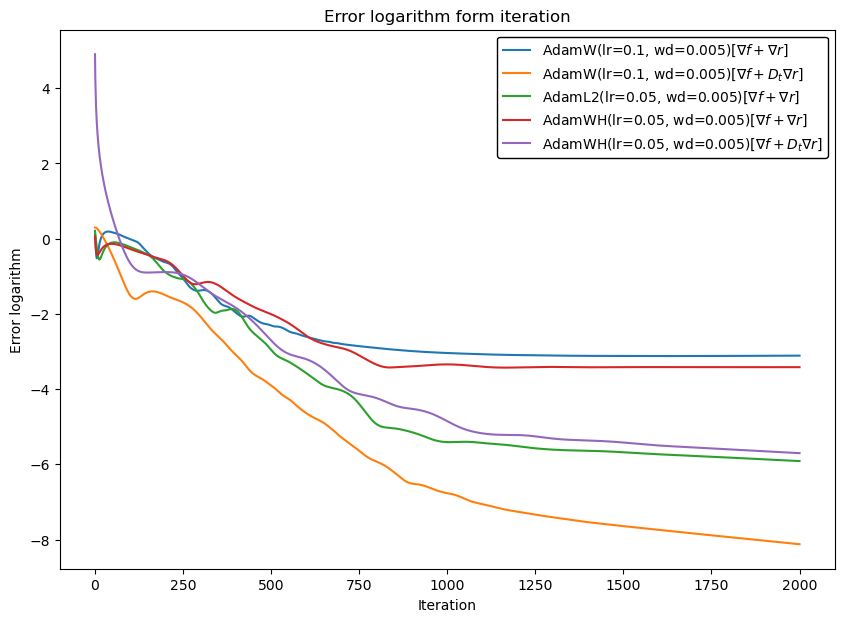
\includegraphics[width=\textwidth]{adams_error.png}
\caption{Adam on dataset mushrooms}
    \label{fig:adams_error}
\end{minipage}
\hfill
\begin{minipage}[h]{0.49\linewidth}
\centering Dataset - mushrooms
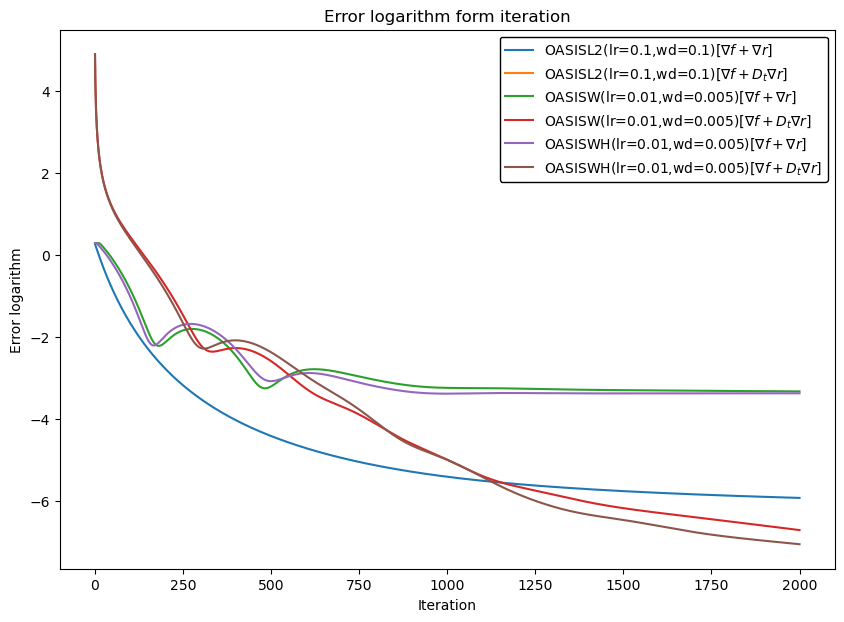
\includegraphics[width=\textwidth]{oasis_error.png}
    \caption{OASIS on dataset mushrooms}
        \label{fig:oasis_error}
\end{minipage}
\label{fig:oasis_error}
\end{figure}
\end{frame}

\begin{frame}{Experiment}

    \begin{figure}[H]
\centering
    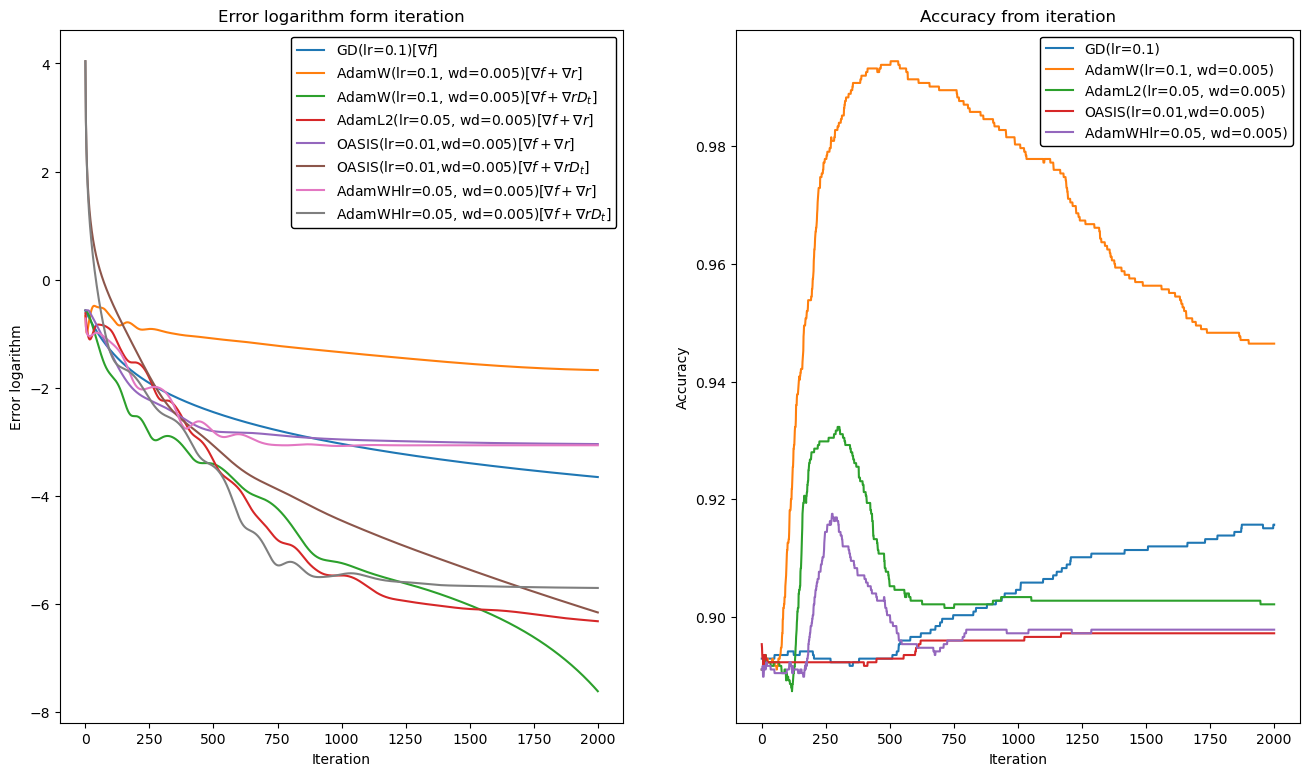
\includegraphics[width=0.75\textwidth]{main_mushrooms.png}
    \caption{Compare different optimization algorithms on dataset: mushrooms}
    \label{fig:main_mushrooms}
\end{figure}
\end{frame}

\begin{frame}{Experiment}
    \begin{figure}[H]
\centering Model - ResNet18, dataset - CIFAR10
    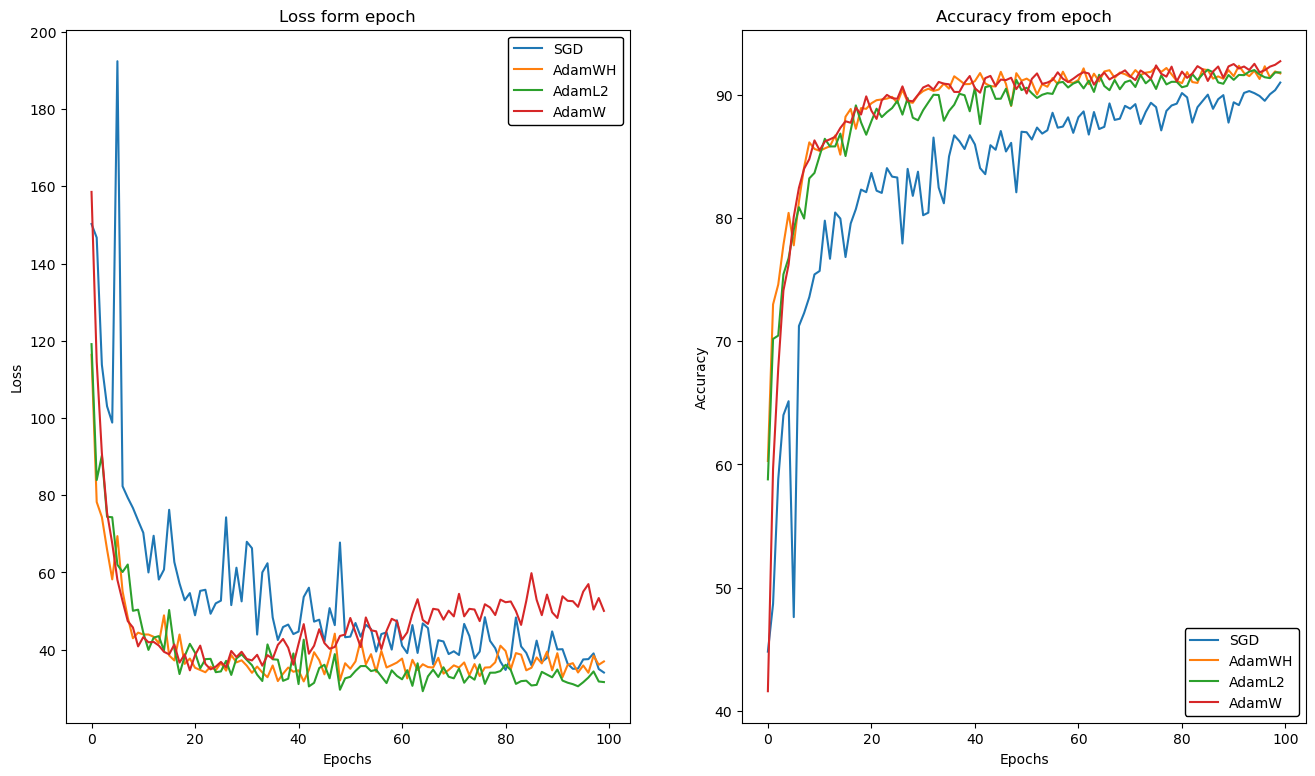
\includegraphics[width=0.75\textwidth]{nn_results.png}
    \caption{Different optimization algorithms on dataset: CIFAR10}

        \label{fig:main_resnet18}
\end{figure}
\end{frame}

\begin{frame}{Publications:}
    \begin{itemize}
        \item Kingma, Diederik P., and Jimmy Ba. "Adam: A method for stochastic optimization." arXiv preprint arXiv:1412.6980 (2014).
        \item Jahani, Majid, et al. "Doubly adaptive scaled algorithm for machine learning using second-order information." arXiv preprint arXiv:2109.05198 (2021).
        \item Sadiev, Abdurakhmon, et al. "Stochastic gradient methods with preconditioned updates." arXiv preprint arXiv:2206.00285 (2022).
        \item Beznosikov, Aleksandr, et al. "On scaled methods for saddle point problems." arXiv preprint arXiv:2206.08303 (2022).
        \item Loshchilov, Ilya, and Frank Hutter. "Decoupled weight decay regularization." arXiv preprint arXiv:1711.05101 (2017).
        \item Xie, Zeke, Issei Sato, and Masashi Sugiyama. "Stable weight decay regularization." (2020).
    \end{itemize}
\end{frame}

\begin{frame}{Conclusion:}
    \begin{itemize}
        \item Proofed the convergence of algorithms with preconditioning with weight decay.
        \item The optimization algorithms AdamW, AdamL2, AdamWH, OASISW, OASISL2, OASISWH, GD on a real problem are investigated on neural networks
        \item Create new optimization algorithm AdamWH.
        \item The optimization algorithms AdamW, AdamL2, AdamW, OASISW, OASISL2, OASISWH, GD on a real problem are investigated on logistic regression.
        \item Investigate optimal learning rates and weight decay.
        \item Choose weight decays less then learning rates.
    \end{itemize}
\end{frame}


\end{document}